\section{Migration}

\subsection{Migration types}

\paragraph{Cold/Offline Migration} is the process of moving a virtual machine from one physical host to another while the virtual machine is powered off. This is the simplest form of migration and is often used for planned maintenance or to move a virtual machine to a different physical host. Cold migration is the most reliable form of migration as there is no risk of data loss or corruption. However, it does require downtime for the virtual machine, which may not be acceptable for some applications.

\paragraph{Hot/Online/Live Migration} is the process of moving a virtual machine from one physical host to another while the virtual machine is still running. This is a more complex form of migration than cold migration, as it requires the virtual machine to be transferred while it is still in use. Hot migration is often used for load balancing, disaster recovery, or to move a virtual machine to a different physical host without downtime. Hot migration is more complex than cold migration and carries a higher risk of data loss or corruption, but it can be performed without downtime for the virtual machine.

\subsection{Migrating between different hypervisors}

% https://pve.proxmox.com/wiki/Migrate_to_Proxmox_VE
\subsubsection{VMware $\rightarrow$ Proxmox}
Proxmox is able to do manual and automatic import of full VMs from ESXi hosts.

\paragraph{Automatic Import}
Proxmox can automatically import VMs from ESXi hosts. VMs with disks on a VMware vSAN storage cannot be imported automatically, but this can be solved by using a small workaround. Just move the disk to a different storage before importing it to Proxmox.
\begin{figure}[H]
    \centering
    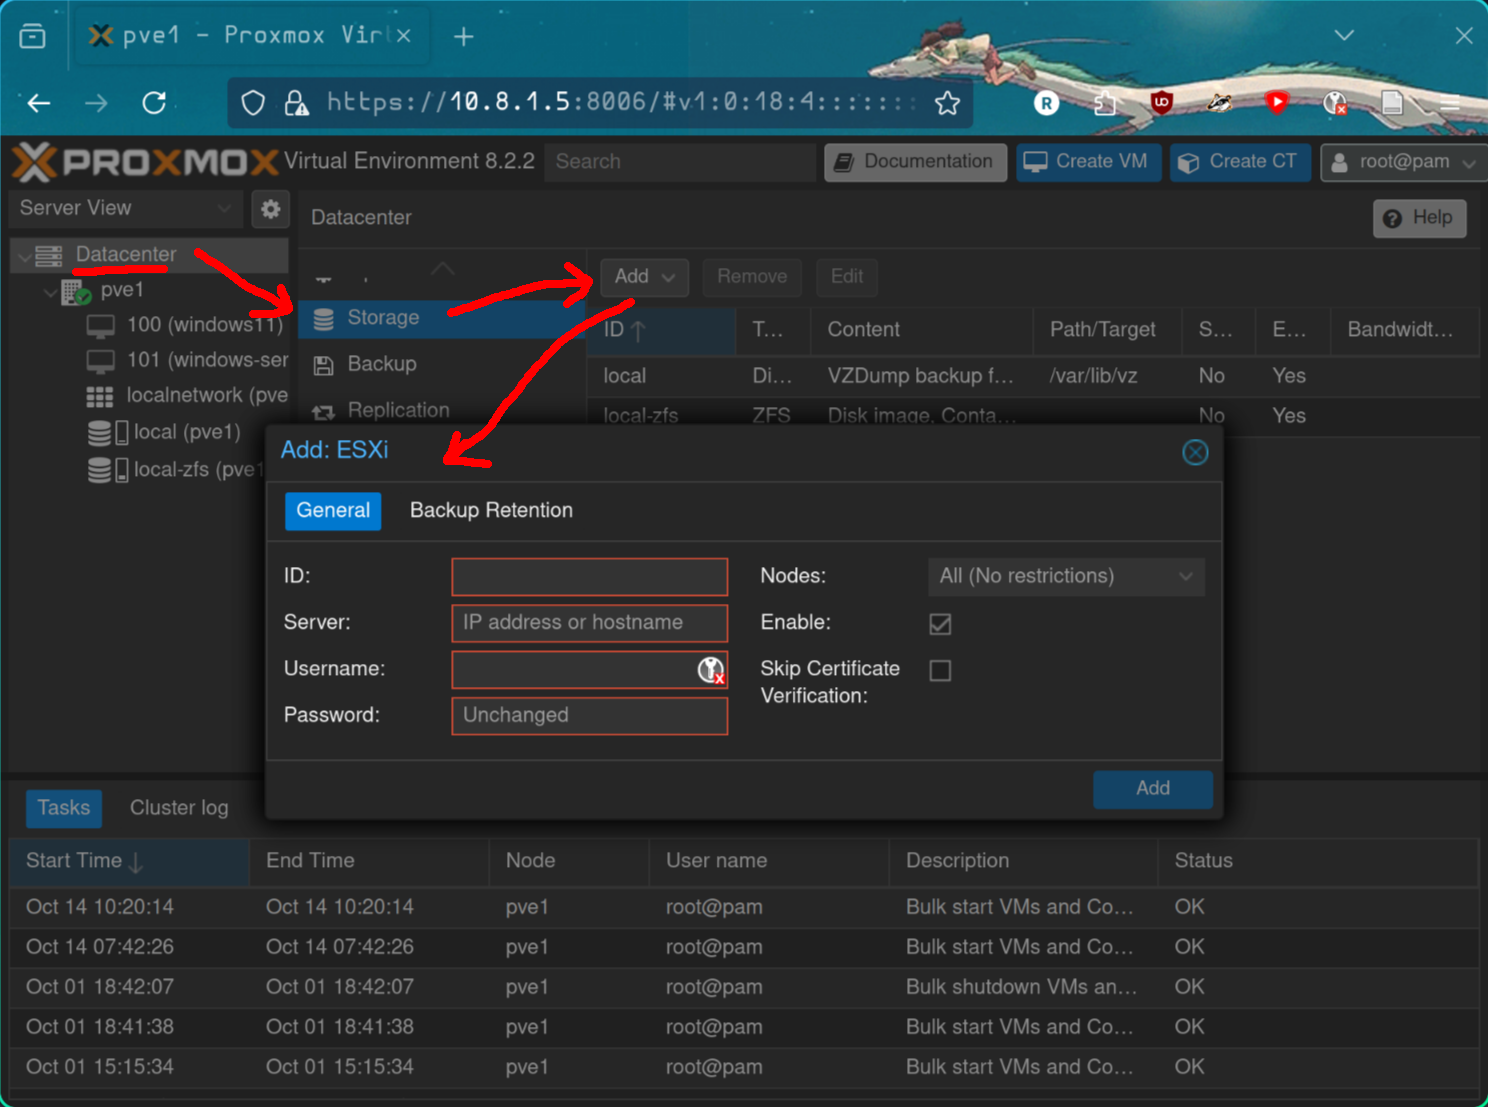
\includegraphics[width=\textwidth]{datacenter_storage_esxi.png}
    \caption{Add ESXi import source to Proxmox}
    \label{fig:proxmox_add_esxi_source}
\end{figure}
To start importing VMs from an ESXi instance it has to be added under Datacenter $\rightarrow$ Storage $\rightarrow$ Add $\rightarrow$ ESXi. \newline
Importing from a vCenter instance is also possible, but will drastically reduce performance.\newline
After adding the ESXi source, the VMs can be imported by selecting the storage in the resource tree and checking the import panel. The VMs can be selected and imported by clicking the import button. You then must select a target storage and network or additionally configure the VM. Now power down the VM on the ESXi host and start the import on Proxmox. The VM will be copied to the Proxmox host and can be started there. You may need to do some post-migration configuration, such as changing the network adapter type or installing VirtIO drivers.

\paragraph{Live Import}
Proxmox also supports live imports. This copies the hard-disk while the VM is still running and syncs all changes asynchronously. When done it automatically starts in Proxmox. While this minimizes downtime it increases the risk of data corruption or loss and is not recommended for production systems.

\paragraph{Mass Imports} should be serialized as much as possible to avoid overloading the ESXi API and potentially interrupting all running imports.
It is generally advised to not import more than 4 VM disks at a time.

\paragraph{Manual Migration}
Manual migration is also possible. The VM must be exported from the ESXi host and then imported to Proxmox. This is more time-consuming and error-prone than automatic migration, but it can be useful for VMs that cannot be migrated automatically.\newline
This can be realized in different ways:
\begin{itemize}
    \item \textbf{Backup} the VM on the ESXi host and restore it on Proxmox.
    \item \textbf{Clone} the VM with a tool like Clonezilla
    \item \textbf{OVF}: Export the VM as an OVF and import it to Proxmox. The \textit{ovftool} can be used to directy import the OVF to Proxmox.
    \item \textbf{Import Disk}: Copy the *.vmdk disk(s) to Proxmox or a shared storage and use the \textit{qm import disk} command to import and convert the disk to the correct target format.
\end{itemize}

\subsubsection{Proxmox $\rightarrow$ VMware}
Migrating VMs from Proxmox to VMware is not as straight forward as the other way around. The VM must be exported from Proxmox and then imported to VMware, as there is no direct import feature in VMware. The following method can be used:
\begin{enumerate}
    \item \textbf{Convert Disk}: The disk must be converted to a format that VMware can read. This can be done with the \textit{qemu-img} tool. 
    e.g. \begin{verbatim}qemu-img convert -f qcow2 -O vmdk disk.qcow2 disk.vmdk\end{verbatim}
    \item \textbf{Create VM}: Next a new VM must be created in VMware which should have the same settings as the VM in Proxmox.
    \item \textbf{Copy Disk}: The converted disk must be copied (e.g. by using scp) to the VMware host and added to the VM. 
    \item \textbf{Boot VM}: The VM can now be started in VMware.
\end{enumerate}

\subsection{Migrating VMs in a cluster}

\subsubsection{Proxmox}
Proxmox supports online/live and offline migration of VMs between nodes in a cluster. 
\paragraph{Preparation} When intending to migrate a virtual machine, it is important to prepare the virtual machine and the target host to ensure a successful migration. The following steps should be taken before migrating a virtual machine:
\begin{itemize}
    \item \textbf{CPU}: Try to choose a CPU-type that is as close to the hardware as possible but supported on all cluster-nodes.
    \item \textbf{Network}: VirtIO NICs are recommended for minimal overhead.
    \item \textbf{Storage}: VirtIO SCSI or VirtIO Block are recommended for minimal overhead. Make sure the target node has enough storage for the VM disk.
    \item \textbf{Memory}: Make sure the target host has enough memory to accommodate the virtual machine.
\end{itemize}

\paragraph{Migrating} to another node can be accomplished by using the CLI or the Web-UI. In the Web-UI it is done by selecting the VM and clicking the migrate button. Disks are either shared or copied early so only the memory and VM state remaing to be synced. The VM will then be moved to another node in the cluster without downtime. Offline migration is also easily possible by shutting down the VM and then migrating it.\newline
Proxmox also supports shared storage, which allows VMs to be migrated between nodes without copying the disk. This is useful for VMs that require high availability or for load balancing. This greatly reduces the time required to migrate a VM, as only the memory and VM state need to be transferred between nodes.

\subsubsection{VMware}
VMware also supports live migration of VMs between hosts in a cluster. This can be accomplished by using vMotion, which allows a VM to be moved between hosts without downtime. vMotion is a complex process that involves transferring the memory and VM state between hosts, as well as updating the network configuration and storage paths. vMotion is a powerful tool that can be used for load balancing, disaster recovery, or planned maintenance. VMware also supports shared storage, which allows VMs to be migrated between hosts without copying the disk.